\documentclass[11pt,letter]{article}
% \include{macro-file}

\def\mainroot{ell_1}

%%%%%% Margins and spacing
\usepackage[top=1in, bottom=1in, left=1in, right=1in]{geometry}
\usepackage{algorithm}
\usepackage{amsmath}
\usepackage{url}
\usepackage{caption}
\usepackage[compact]{titlesec}
%\usepackage{bm}
\usepackage{txfonts} %\usepackage{times}
\usepackage{color}
\usepackage{tikz}
\usetikzlibrary{calc}
\usepackage{cancel}
\usepackage{soul}
\usepackage{graphicx}
\usepackage{caption}
\usepackage{subcaption}
\usepackage{algpseudocode}

\usepackage{sidecap}
\sidecaptionvpos{figure}{c}

\usepackage{enumitem}
\setlist{nolistsep}

%\setcounter{MaxMatrixCols}{20}

\newcommand\mjsnote[1]{{\bf [#1 -mjs]}}

\newcommand{\meas}{{\mathbf \mu}}
\newcommand{\tightpgh}[1]{\vskip 3pt\noindent\textbf{#1}}
\newcommand{\signalw}{{\mathbf w}}
\newcommand{\signalx}{{\mathbf x}}
\newcommand{\signaly}{{\mathbf y}}
\newcommand{\signalz}{{\mathbf z}}

%\expandafter\def\expandafter\normalsize\expandafter{%
%    \normalsize
%    \setlength\abovedisplayskip{2pt}
%    \setlength\belowdisplayskip{2pt}
%    \setlength\abovedisplayshortskip{0pt}
%    \setlength\belowdisplayshortskip{0pt}
%}\makeatother
%
%\renewcommand\floatpagefraction{.9}
%\renewcommand\topfraction{.9}
%\renewcommand\bottomfraction{.9}
%\renewcommand\textfraction{.1}   
%\setlength{\textfloatsep}{10pt plus 1.0pt minus 2.0pt}

% Jian \DeclareMathOperator*{\median}{median}
\newcommand{\mb}{\ensuremath\mathbf}
\newcommand{\F}{\ensuremath\mathbb{F}}

\title{UI for RNA-seq quantification \footnote{Course Project Report of CSE 549.}}
\author{
%\alignauthor
xxxx xxxxx\\
       {\small SBU ID: xxxxxx}\\
       {\small Department of Computer Science}\\
       {\small Stony Brook University} \\
       {\small \texttt{xxxxx@cs.stonybrook.edu}}
%\alignauthor
\and
xxxx xxxxx \\
       {\small SBU ID: xxx}\\
       {\small Department of Computer Science}\\
       {\small Stony Brook University} \\
       {\small \texttt{xxxxx@cs.stonybrook.edu}}
%\alignauthor
\and
xxxx xxxxxx \\
       {\small SBU ID: xxx}\\
       {\small Department of Computer Science}\\
       {\small Stony Brook University} \\
       {\small \texttt{xxxxx@cs.stonybrook.edu}}
%\alignauthor
\and
%\alignauthor
Jian Yang \\
       {\small SBU ID: 110168771}\\
       {\small Department of Computer Science}\\
       {\small Stony Brook University}\\
       {\small \texttt{yang16@cs.stonybrook.edu}}
}
\date{}


\raggedbottom

\begin{document}
\maketitle

\begin{abstract}
Write the abstraction Here
\end{abstract}

\thispagestyle{empty}
\newpage
\addtocounter{page}{-1}

\section{Introduction}
write the introduction here. \\

\newpage
\section{Mean-Variance Analysis of k-clique}\label{sec:var}
In this section, we would analyze the mean, the variance and the related bounds of DOULION method's affect to calculate $k$-clique. Here we would not try to find the maximum possible $k$ in a graph but to analyze the statistics properties of a fixed $k$.
\subsection{Mean of k-clique}
Let $m$ be the number of $k$-cliques in the original graph. To calculate the mean of random sampling with DOULION, here is the calculation.\\
\[
        \begin{split}
Mean(k\text{-clique}) &= E[X] = E[\sum_{i=1}^{m} \frac{1}{p^{\binom{k}{2}}} \delta_i] = \frac{1}{p^{\binom{k}{2}}} \sum_{i=1}^{m}  E[\delta_i] \\
&= \frac{1}{p^{\binom{k}{2}}} \sum_{i=1}^{m} p^{\binom{k}{2}} \\
&= m
        \end{split}
\]
From the result we could see the expected value of the random sampling is same as the value without the random sampling. That indicates the random sampling wouldn't change the expected value of $k$-clique counting.
\subsection{Variance of k-clique}
To calculate the variance of $k$-clique counting with random sampling, here is the calculation. \\
\[
        \begin{split}
Var(k-clique) &= Var( \frac{1}{p^{\binom{k}{2}}} \sum_{i=1}^{m} \delta_i ) = \frac{1}{p^{k(k-1)}} \sum_{i=1}^{m} \sum_{j=1}^{m} Cov(\delta_i, \delta_j) \\
&= \frac{1}{p^{k(k-1)}}(m(p^{k(k-2)/2} - p^{k(k-1)}) + 2\sum_{l=2}^{k-1} N_{k,l}(p^{k(k-1)-l(l-1)/2} - p^{k(k-1)}))
        \end{split}
\]
Where $N_{k,l}$ presents the number of two $k$-cliques sharing $l$ common vertices. \\
From this result, we could see that the variance is quite large, for example, one term of it is $\frac{1}{p^{k(k-1)}}(m(p^{k(k-2)/2} - p^{k(k-1)})) = m(\frac{1}{p^{k(k-2)/2}}-1)$. Since we know that $p < 1$, so $m(\frac{1}{p^{k(k-2)/2}}-1) \gg m$. We would see more about how large the variance bound is in the next sub section.

\subsection{Theoretical Bound}
In this part we would try to calculate the Chebyshev's bound by Chebyshev's inequality\cite{cheby} \cite {cheby_wki}. \\
\[
        \begin{split}
Pr(|X - m| \geq \epsilon m) &\leq \frac{Var(X)}{\epsilon^2 m^2}  \\
&= \frac{1}{p^{k(k-1) \epsilon^2 m^2}}(m(p^{k(k-2)/2} - p^{k(k-1)}) + 2\sum_{l=2}^{k-1} N_{k,l}(p^{k(k-1)-l(l-1)/2} - p^{k(k-1)}))
        \end{split}
\]
Actually this is a quite bad bound. For example, when $k = 4, p=0.1, \epsilon = 0.1$, if $m < 10^8$, it's always hold that $Pr(|X - m| \geq \epsilon m) > 1$, which is obviously true because it's a probability with a random variable. The Chebyshev bound really tells nothing because the theoretical variance is too large.
\subsection{Upper Bound}
From the variance's equation, we could see that it includes two part without the common factor $\frac{1}{p^{k(k-1)}}$ if both $p$ and $k$ are fixed. The first part is $m(p^{k(k-2)/2} - p^{k(k-1)})$ which is dependent only with m while the second term  $2\sum_{l=2}^{k-1} N_{k,l}(p^{k(k-1)-l(l-1)/2} - p^{k(k-1)})$ is dependent with $N_{k,l}$. \\
For an arbitrary graph with $m$ $k$-cliques, if there is a complete graph with the same number $m'$ of $k$-clique with the equation $m' = m$, it's obviously that for the complete graph, all the numbers of shared vertices $N'_{k,l} \geq N_{k,l}$. So we could make this complete graph's variance as the upper bound of the variance of a graph with the number $m$ of $k$-clique.
\subsection{Upper Bound Experiments}
Since we have the upper bound of the variance as a complete graph with the same number of $k$-cliques, I did the following experiments to test $k$-clique's variance on a complete graph with 100 vertices. The random sampling and the counting has run for 100 rounds and the number is calculated with the average of the results from all rounds. \\

\begin{figure}[h!]
\centering
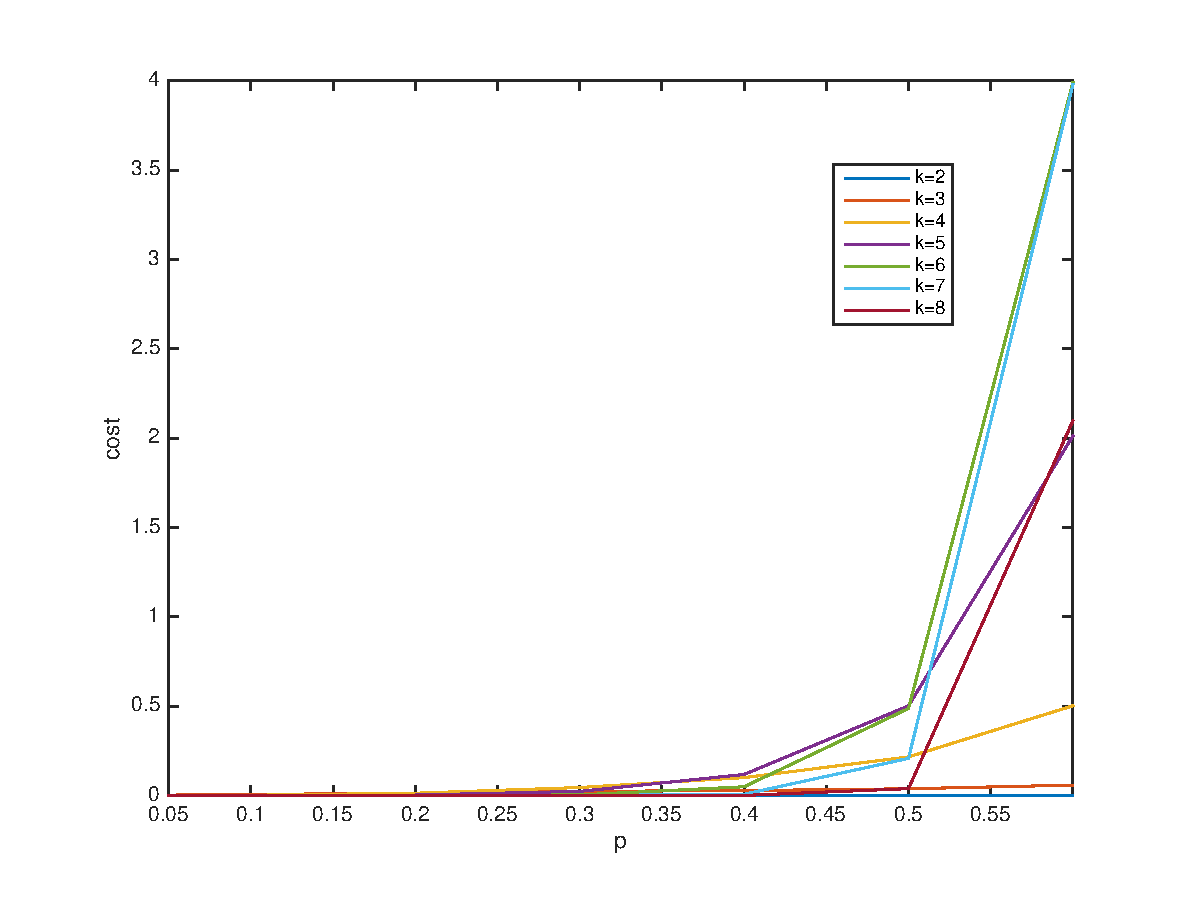
\includegraphics[width=5in]{fig/cost.eps} % [height=2.5in, width=3.5in]
\caption{Cost of $k$-clique on a complete graph}
\label{fig:perf}
\end{figure}

\begin{figure}[h!]
\centering
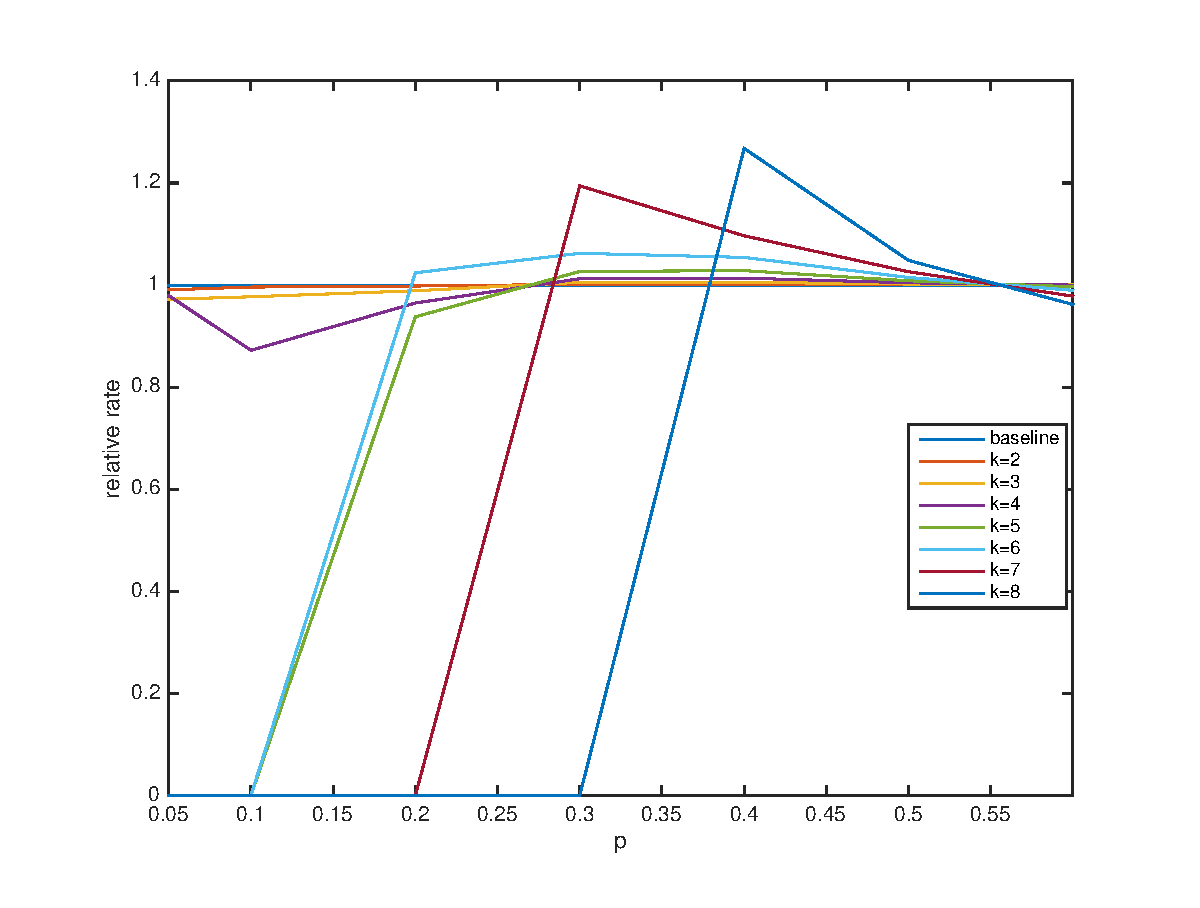
\includegraphics[width=5in]{fig/mean.eps} % [height=2.5in, width=3.5in]
\caption{Mean of $k$-clique on a complete graph}
\label{fig:mean}
\end{figure}

\begin{figure}[h!]
\centering
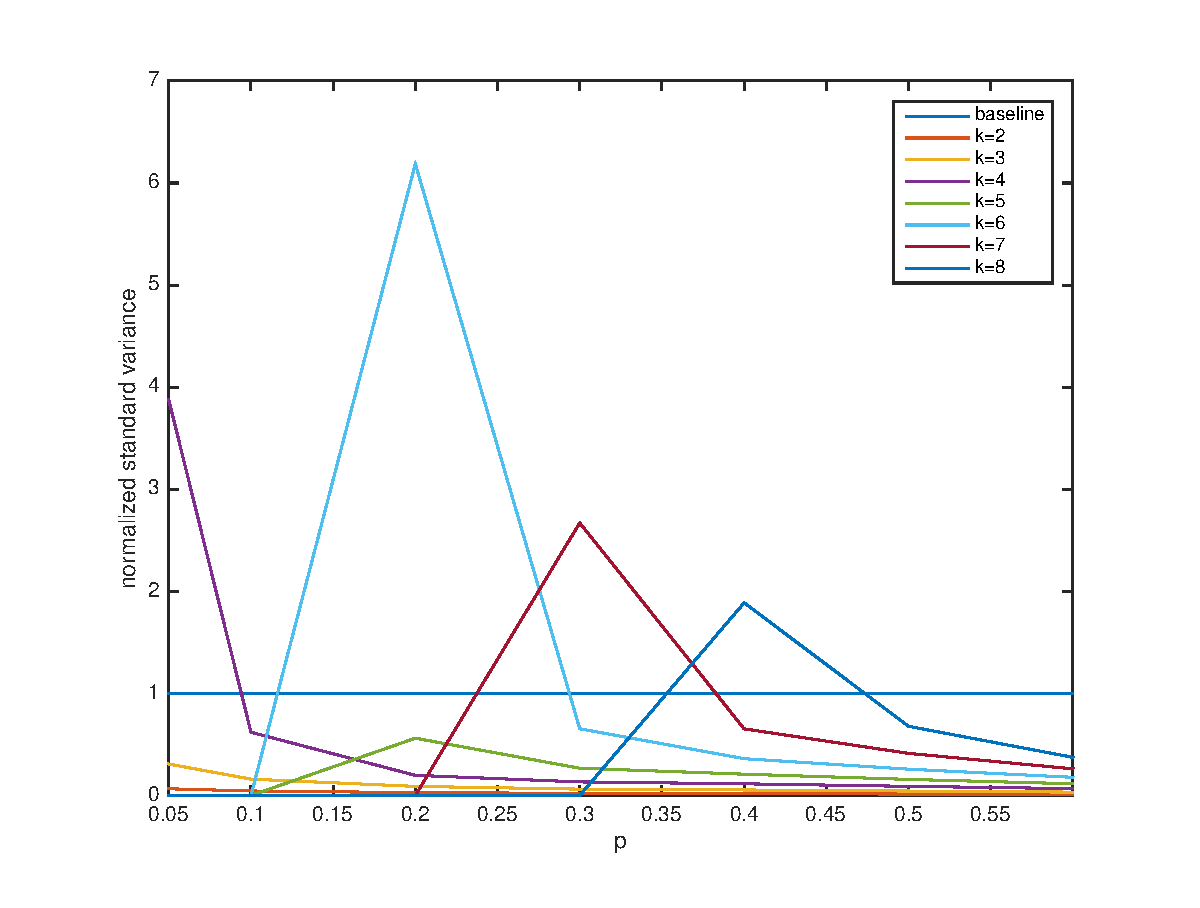
\includegraphics[width=5in]{fig/variance.eps} % [height=2.5in, width=3.5in]
\caption{Variance of $k$-clique on a complete graph}
\label{fig:perf}
\end{figure}

In these 3 figures, the $x$-axis is same as the number of . In each figure, we would draw different lines for different $k$ values from 2 to 8. \\
The performance is shown as Figure \ref{fig:perf}. It's obviously the performance increases rapidly. Theoretically it would be exponential and the figure is almost showing that. The performance of a complete graph doesn't have close relation with an arbitrary graph with the same number of $k$-clique, because the number of the vertices and edges are also important factors of the performance. \\
The mean is shown as Figure \ref{fig:mean}. From the figure we could see that the mean of the result converges to the real value quickly. \\
The normalized standard variance is shown as Figure \ref{fig:variance}. From the figure we could see that the variances quickly converge. For example, the line $k=8$, we could see that when $p = 0.5$, the variance is 0.6782 and it's under 1. \\
As a conclusion, we could see that from this experiment, when $k$ is large( $k > 5$), the normalized standard variances still converge quickly when $p = 0.5$. Generally, considering the cost of the running, we would see that, for $k = 8, p=0.5$, the ratio of the cost of the DOULION comparing with the original cost is: \\
\[
        \begin{split}
ratio(DOULION) &= \frac{\text{Sampled Cost}}{\text{Original Cost}} \\
&= \frac{(\text{Original Cost}) \cdot p^k \cdot rounds}{\text{Original Cost}} \\
&=  p^k \cdot rounds \\
&= 0.5^8 \cdot 100 = \frac{100}{256} \approx 0.39
        \end{split}
\]
So the speedup is $1/0.39 = 2.56$. Which means we could get one 2.5X speedup to get the approximate result with normalized standard variance's upper bound is 0.6782 for $k=8, p = 0.5$. This is not large but valuable. But if we could accept the upper bound of the normalized standard variance as 1.8881, the speed up would be $1/(0.4^8 \cdot 100) \approx 15$. \\
Come back to the case for $k=8, p = 0.5$. If we what $Pr(|X - m| \geq \epsilon m)  \leq 0.01$, we need to set $\frac{Var(X)}{\epsilon^2 m^2} = 0.01$. And from the standard normalized variance we know that $\frac{Var(X)}{m^2} \leq 0.6782$. So we have: \\
\[
        \begin{split}
Pr(|X - m| \geq \epsilon m)  &\leq \frac{Var(X)}{\epsilon^2 m^2} \leq \frac{0.6782}{\epsilon^2}
        \end{split}
\]
Let $ \frac{0.6782}{\epsilon^2} = 0.01$, we have $\epsilon = 8.24$. Which means we have one 9-approximate algorithm with 2.5-fold speed up comparing the brute-force counting. Similarly we could calculate we could have one 15-approximate algorithm with 15-fold speedup if we set $p = 0.4$. And we could have one 17-approximate algorithm with 45-fold speed up if $k = 7, p = 0.3$.

\subsection{Conclusion}
From the theoretically analysis and the experiment of the upper bound, we found that this sampling algorithm would bring huge variance for $k$-clique counting if $k$ is large. But from the experiment of the upper bound, we could also see that we could get an approximate for the original algorithm. If we just want to know a general range of the number of $k$-clique, this would be useful somehow.

\subsection{Improvement}
One thing I saw is that, it might be possible to use the first 4 moments of $Pr(X \geq a) = Pr(e^{tX} \geq e^{ta})$ while Chernoff bound is just using the first two moments.

\section{Clustering and Community Detect with Random Sampling}\label{sec:cluster}
\subsection{Introduction}
Clustering and community detect are important tasks in network study. In this section, I would introduce how to use random sampling to get a faster algorithm to clustering and community detection. \\
The intuitions are, with high probability the random sampling could keep high density sub graphs still connected after random sampling, and the communities are also kept in high probability. \\
In nowadays, the methods to clustering and community detection are various but all the methods at least linear to the number of edges if the graph is sparse.

% Calculate Laplacian Matrix?s eigenvectors
% Arnoldi-Lanczos iterative algorithm
% At least O(|E||V|2) or O(|E||V|log|V|)
% DOULION
% Remove (1-1/p) |E| for uniformly sampling
% Dangling Vertices to reduce |V|

\subsection{Algorithm}

\begin{algorithm} [h!]                     % enter the algorithm environment
\caption{Sentence Similarity Calculation based on Wordnet}          % give the algorithm a caption
\label{alg:same}                           % and a label for \ref{} commands later in the document
\begin{algorithmic} [1]                   % enter the algorithmic environment
 \ForAll {$v \in G$'s vertices}
   \State {add $v$ to $G'$}
 \EndFor
 \ForAll {$e \in G$'s edges}
   \State {$result \gets $ flip a coin with probability $p$}
   \If {$result = Head$}
     \State {add $e$ to $G'$}
   \EndIf
 \EndFor
 
 \State {$labels \gets$ spectral clustering and $k$-mean's clustering result}
 \State {Apply $labels$ to $G$}
 \ForAll {$v \in G$'s vertices}
   \State {$label(v) \gets $ majority label of $v$'s neighbors on $G$}
 \EndFor
\end{algorithmic}
\end{algorithm}

The algorithm is shown as Algorithm \ref{alg:same}. It includes the following parts:
\begin{enumerate}
\item Build a sparsed graph with random sampling on the original graph.
\item Run spectral clustering and $k$-mean clustering on the sparsed graph $G'$.
\item Use majority vote by using the neighbors connections on original graph $G$ to do justification each vertex's label.
\end{enumerate}
The purpose of the 3rd step is to assume most of the nodes are labeled correctly for the sparsed graph, and then use one naive method to greedily do the justification to reduce errors.

\subsection{Experiment}
The experiment example is shown as Figure \ref{fig:cluster}. The parameter $p$ is set as 0.2. Each community is labelled as different colors. The connection inside one community is colored with the community color and the connection between two different communities is colored with yellow color. \\
Figure \ref{fig:origin} shows the $k$-mean clustering results on the original graph. There are 4 communities in the original graph. \\
Figure \ref{fig:kmean} shows the community detection result after the sparse, spectral clustering and $k$-mean clustering. There are also 4 communities. And we could see most of the vertices are labelled as the same community with the original graph but there are still several errors. For example, the red lines connecting the red community and the green community indicates some vertex in green community was wrongly labelled to red community. \\
Figure \ref{fig:vote} shows the result after majority vote justification. We could see the result is almost same as the original community labelling. The accuracy is 96\% comparing with the original results, and the speed up is 5-fold because we chose $p = 0.2$.
\begin{figure}[h!]
        \centering
        \begin{subfigure}[h]{0.5\textwidth}
                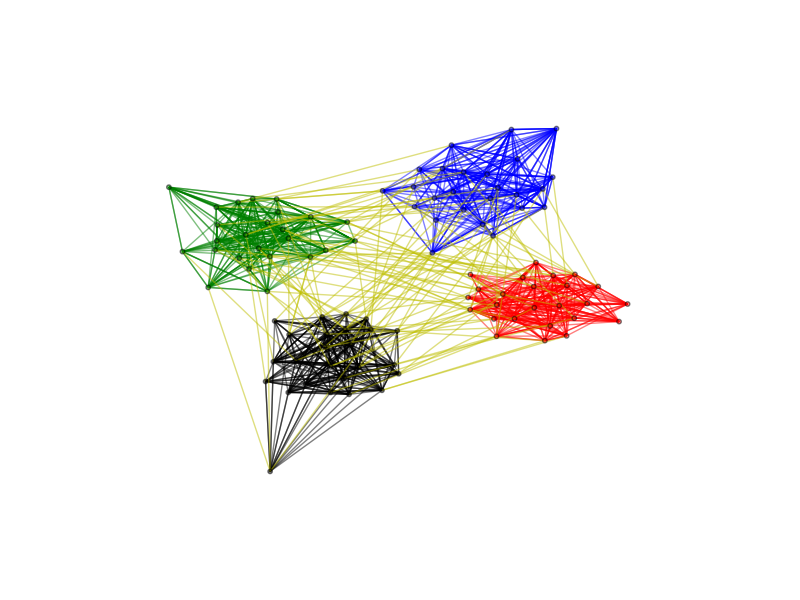
\includegraphics[width=\textwidth]{fig/221.png}
                \caption{Original Network Graph}
                \label{fig:origin}
        \end{subfigure}%
        \begin{subfigure}[h]{0.5\textwidth}
                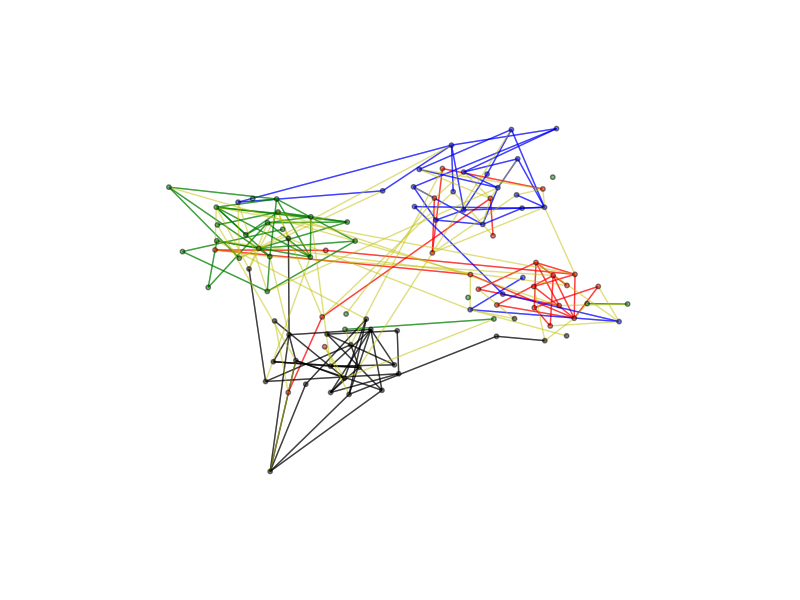
\includegraphics[width=\textwidth]{fig/222.png}
                \caption{Clustered Result with Random Sampling Graph}
                \label{fig:kmean}
        \end{subfigure}
        %add desired spacing between images, e. g. ~, \quad, \qquad, \hfill etc.
          %(or a blank line to force the subfigure onto a new line)
          
        \begin{subfigure}[h]{0.5\textwidth}
                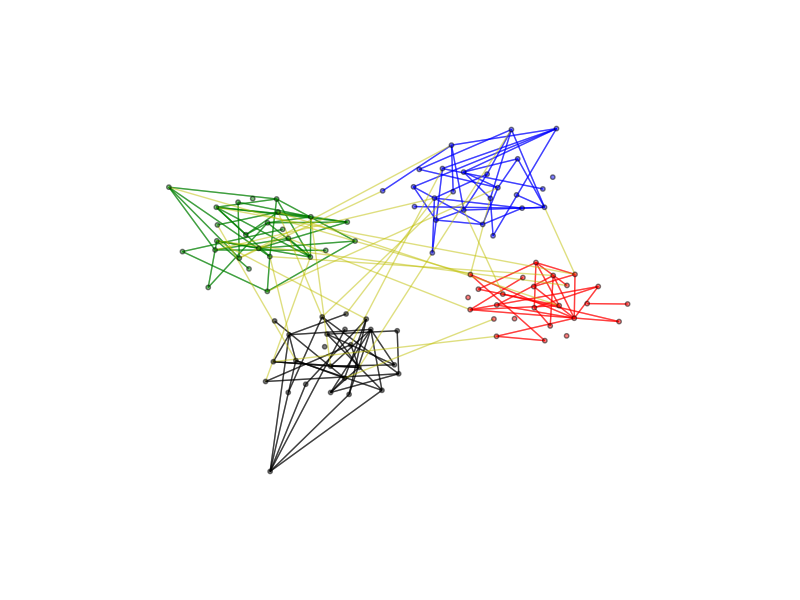
\includegraphics[width=\textwidth]{fig/223.png}
                \caption{After Justification with Majority Vote}
                \label{fig:vote}
        \end{subfigure}
        \caption{Pictures of Clustering with Random Sampling}\label{fig:cluster}
\end{figure}

\subsection{Conclusion}
From the experiment result, we could see that the result is quite good. With random sampling, the speed up is high and the accuracy is close to 100\%. This verified my intuition that the sparsing with random sampling would make the sparsed graph has almost similar communities with the original graph. And we could easily get better accuracy by the majority vote justification method.

\subsection{Improvement}
Since the art-of-state algorithms to cluster and detect the community are complicated as iteration algorithms without fixed complexity, there is still more complicated theoretical analysis for the speed up and the accuracy. We should also do the experiments on different types of networks to see if there is some corner cases for the sparsing. \\
Another method which may bring a better accuracy is sampling with weighted and this should keep the critical edges with higher probability which may be helpful in this methodology.


\newpage
\section{Graph Cut with two methods of Sampling} \label{sec:div}
\subsection{Introduction}
Graph Cut is a popular problem in graphic analysis. The Similarity Matrix could be used for graph cut as studied by Jianbo Shi et al \cite{shi}. One popular sparse method for Similarity Matrix is Effective Resistance introduced by Richard Peng et al\cite{peng}. \\
In this section, I implemented two methods to sparse the graph. One is the stable sampling and another method is random sampling.  And with the sparsed methods, I would follow Jianbo Shi's framework\cite{shi} for graph cut. \\
The intuition is that if the sparsing still keeps the basic outlines of the original graph if we sparse the graph carefully. \\

% Classic Sparse method: Effective Resistance
% Classic Object to study: Similarity Matrix
% Study by Richard Peng et al.
% Classic Application: graph cut
% Study by Jianbo Shi et al.
% Sparse Similarity Matrix
\subsection{Algorithm of Stable Sampling}
For Stable Sampling, there is one parameter as the sparse ratio as $d$. Let the length and width of the original graph be $L$ and $W$, the sparsed graph's size would be $L/d$ and $W/d$, which means we would get a sample graph with the $1/d^2$ pixels comparing the original graph. \\
The algorithm is shown as Algorithm \ref{alg:stable_sample}
\begin{algorithm}[h!]                      % enter the algorithm environment
\caption{Graph Cut with Stable Sampling}          % give the algorithm a caption
\label{alg:stable_sample}                           % and a label for \ref{} commands later in the document
\begin{algorithmic} [1]                   % enter the algorithmic environment
\Require {$d$, $G$}
 \For {$i \gets 0 $ to $L/d$}
   \For {$j \gets 0 $ to $W/d$}
     \State {$G'[i][j] \gets \frac{\sum_{k=0}^{d-1} \sum_{l=0}^{d-1} G[i \cdot d + k][j \cdot d + l] }{d^2}$}
   \EndFor
 \EndFor
 \State {$affinity\_matrix \gets $ build affinity matrix on $G'$}
 \State {$labels' \gets $ labels of spectral clustering on $affinity\_matrix$}
 \For {$i \gets 0 $ to $L$}
   \For {$j \gets 0 $ to $W$}
     \State {$labels[i][j] \gets labels'[\lfloor i/d \rfloor][\lfloor j/d \rfloor]$}
   \EndFor
 \EndFor
 \State \Return {$labels$}
\end{algorithmic}
\end{algorithm}

\subsection{Algorithm of Random Sampling}
The algorithm of random sampling is shown as Algorithm \ref{alg:random_sample} .
\begin{algorithm}[h!]                      % enter the algorithm environment
\caption{Graph Cut with Random Sampling}          % give the algorithm a caption
\label{alg:random_sample}                           % and a label for \ref{} commands later in the document
\begin{algorithmic} [1]                   % enter the algorithmic environment
\Require {$p$, $G$}
 \State {$affinity\_matrix \gets $ build affinity matrix on $G$}
 \ForAll {non-zero element $\in affinity\_matrix$}
   \State {$result = $ flip a coin with probability $p$}
   \If {$result = Head$}
     \State {set the element to be 0 in the $affinity\_matrix$}
     \State {set the symmetric element to be 0 in the $affinity\_matrix$}
   \EndIf
 \EndFor
 \State {$labels \gets $ labels of spectral clustering on $affinity\_matrix$}
 \State \Return {$labels$}
\end{algorithmic}
\end{algorithm}

\subsection{Experiment of Stable Sampling}

The experiment of stable sampling is shown as Figure \ref{fig:graphcut}. Figures \ref{fig:graphcut_5}, \ref{fig:graphcut_10}, \ref{fig:graphcut_20} show the graph cut results for 5, 10, 20 areas on the original graph. Figures \ref{fig:graphcut_small4_5}, \ref{fig:graphcut_small4_10}, \ref{fig:graphcut_small4_20} show the graph cut results for 5, 10, 20 areas on the graph with 16-fold sparsed. And Figures \ref{fig:graphcut_small_5}, \ref{fig:graphcut_small_10}, \ref{fig:graphcut_small_20} show the graph cut results for 5, 10, 20 areas on the graph with 100-fold sparsed.\\
First, we would look at the graph cut results. We could see even for the 100X graph, the results are still good. The plaster figure is detected in all the graphs for 16X and 100X. The desk lamp is also detected in all graphs for 16X and 100X when the number of area is 20. In the 100X graph, the desk lamp's scope is better than others. The plaster figure detections are better for 16X and 100X than the detection in the original graph. \\
Second, we would look at the performance. The speed up ratios are shown in Table \ref{table:speedup}. The cost increases rapidly when the number of areas is small but with stable sampling, we could get at most 6,243-fold speed up which is quite amazing.

\begin{figure}[h!]
        \centering
        \begin{subfigure}[h]{0.33\textwidth}
                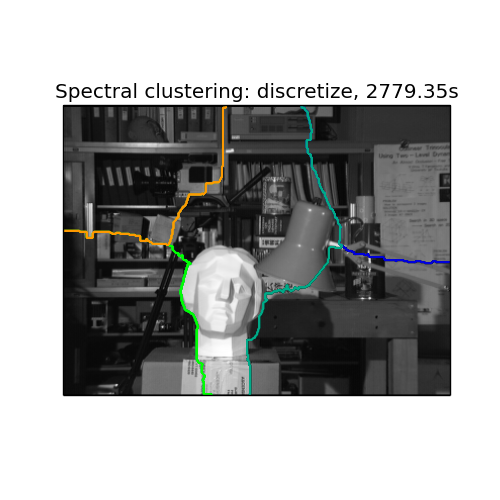
\includegraphics[width=\textwidth]{fig/592_large_5.png}
                \caption{Graph Cut to 5 areas on Original Graph}
                \label{fig:graphcut_5}
        \end{subfigure}%
        \begin{subfigure}[h]{0.33\textwidth}
                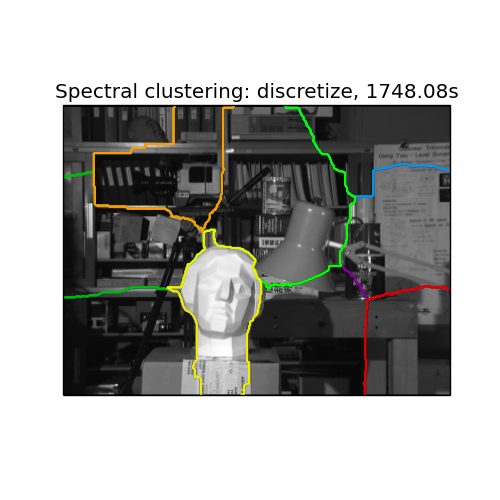
\includegraphics[width=\textwidth]{fig/592_large_10.png}
                \caption{Graph Cut to 10 areas on Original Graph}
                \label{fig:graphcut_10}
        \end{subfigure}
        \begin{subfigure}[h]{0.33\textwidth}
                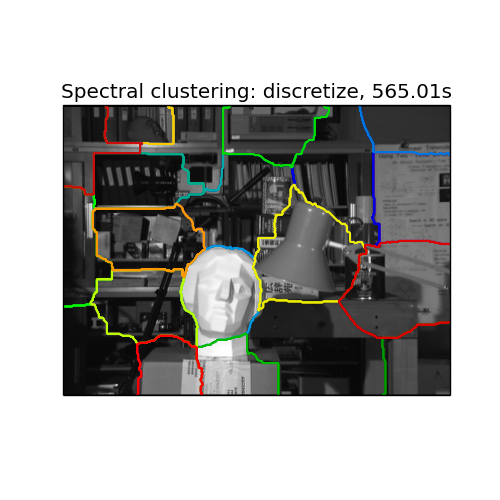
\includegraphics[width=\textwidth]{fig/592_large_20.png}
                \caption{Graph Cut to 20 areas on Original Graph}
                \label{fig:graphcut_20}
        \end{subfigure}
        
        \begin{subfigure}[h]{0.33\textwidth}
                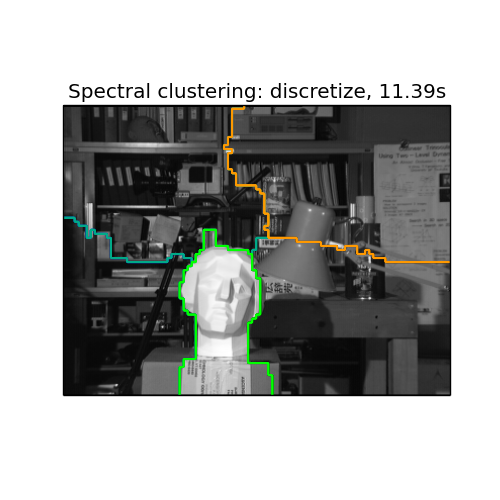
\includegraphics[width=\textwidth]{fig/592_small4_5.png}
                \caption{Graph Cut to 5 areas on 16X Graph}
                \label{fig:graphcut_small4_5}
        \end{subfigure}%
        \begin{subfigure}[h]{0.33\textwidth}
                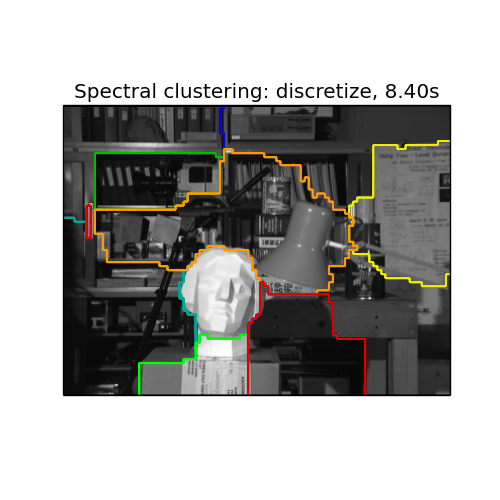
\includegraphics[width=\textwidth]{fig/592_small4_10.png}
                \caption{Graph Cut to 10 areas on 16X Graph}
                \label{fig:graphcut_small4_10}
        \end{subfigure}
        \begin{subfigure}[h]{0.33\textwidth}
                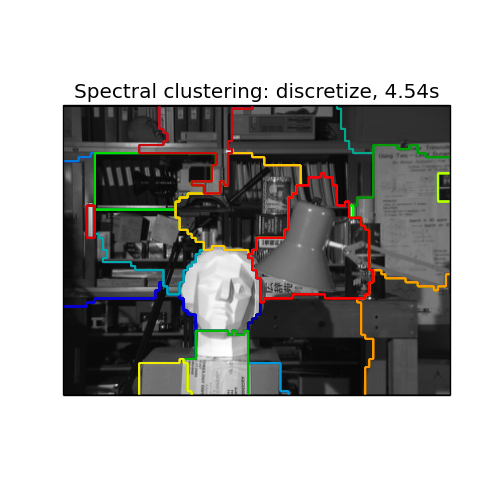
\includegraphics[width=\textwidth]{fig/592_small4_20.png}
                \caption{Graph Cut to 20 areas on 16X Graph}
                \label{fig:graphcut_small4_20}
        \end{subfigure}
        
        \begin{subfigure}[h]{0.33\textwidth}
                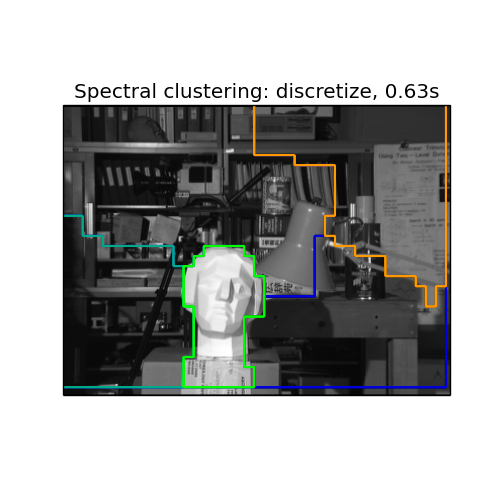
\includegraphics[width=\textwidth]{fig/592_small_5.png}
                \caption{Graph Cut to 5 areas on 100X Graph}
                \label{fig:graphcut_small_5}
        \end{subfigure}%
        \begin{subfigure}[h]{0.33\textwidth}
                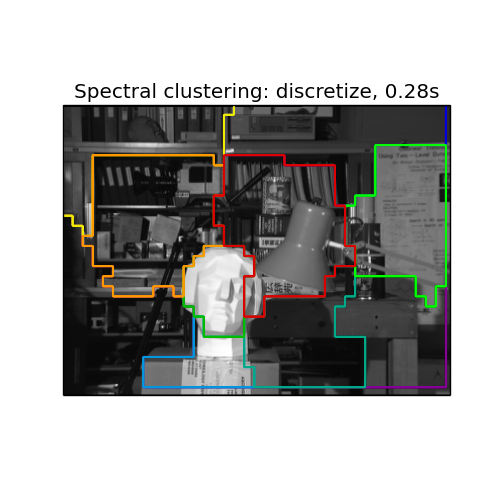
\includegraphics[width=\textwidth]{fig/592_small_10.png}
                \caption{Graph Cut to 10 areas on 100X Graph}
                \label{fig:graphcut_small_10}
        \end{subfigure}
        \begin{subfigure}[h]{0.33\textwidth}
                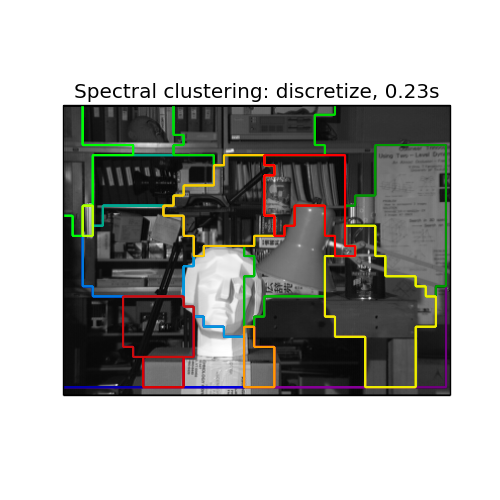
\includegraphics[width=\textwidth]{fig/592_small_20.png}
                \caption{Graph Cut to 20 areas on 100X Graph}
                \label{fig:graphcut_small_20}
        \end{subfigure}
        \caption{Pictures of Clustering with Random Sampling}\label{fig:graphcut}
\end{figure}

\begin{table*}[h!]
{\centering\footnotesize
\begin{tabular}{|c|r|r|r|}
\hline
number of areas & 5 & 10  & 20 \\ \hline
16X graph & 244.02 & 208.10 & 124.45 \\ \hline
100X graph & 4411.67 & 6243.14 & 2456.57 \\ \hline
\end{tabular}
\captionsetup{font=footnotesize,labelfont=bf}
\caption{Speed up ratios for Stable Sampling}
\label{table:speedup}
}
\end{table*}

\subsection{Experiment of Random Sampling}
The results in this part are not so good as stable sampling. Figures \ref{fig:graphcut_random_01_10} and \ref{fig:graphcut_random_05_10} are the results with random sampling parameter $p = 0.1$ and $p = 0.5$. Both of the results are not good and only the general skeletons are ok. \\
There are 4-fold speed up for $p = 0.1$ and 2.6-fold speed up for $p = 0.5$. This is a not bad performance but not good because of the poor accuracy.
\begin{figure}[h!]
        \centering
        \begin{subfigure}[h]{0.48\textwidth}
                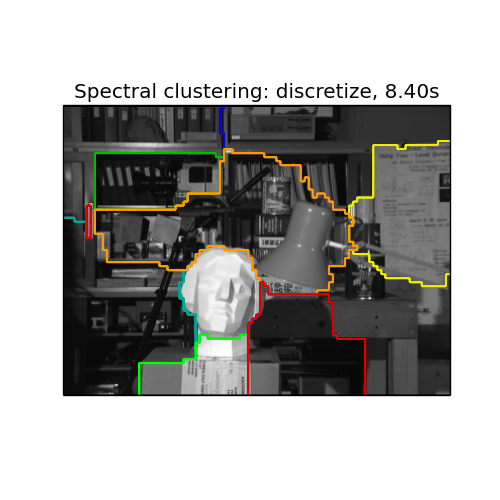
\includegraphics[width=\textwidth]{fig/592_small4_10.png}
                \caption{Graph Cut to 10 areas on 16X Graph}
                \label{fig:graphcut_random_small4_10}
        \end{subfigure}
        \begin{subfigure}[h]{0.48\textwidth}
                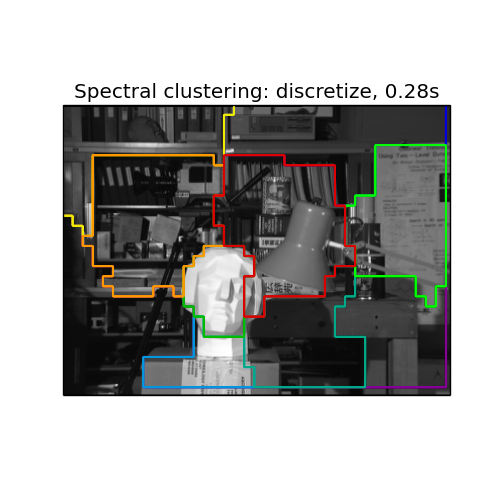
\includegraphics[width=\textwidth]{fig/592_small_10.png}
                \caption{Graph Cut to 10 areas on 100X Graph}
                \label{fig:graphcut_random_small_10}
        \end{subfigure}
        
        \begin{subfigure}[h]{0.48\textwidth}
                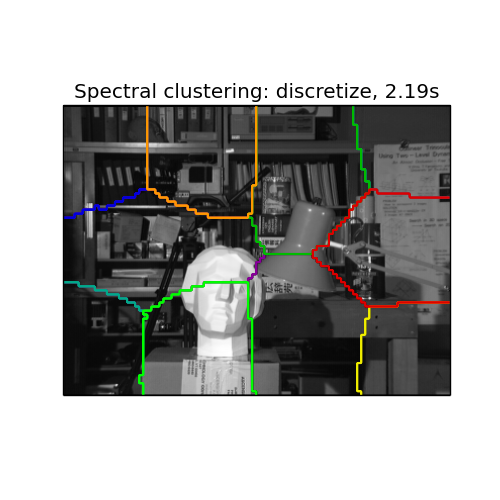
\includegraphics[width=\textwidth]{fig/592_random_0_1_10.png}
                \caption{Graph Cut to 10 areas on 16X Graph with $p = 0.5$}
                \label{fig:graphcut_random_01_10}
        \end{subfigure}
        \begin{subfigure}[h]{0.48\textwidth}
                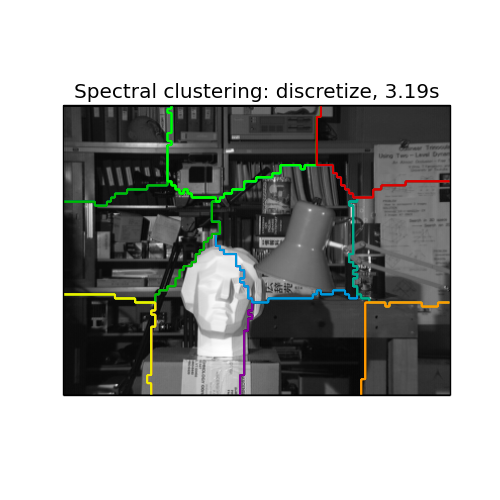
\includegraphics[width=\textwidth]{fig/592_random_0_5_10.png}
                \caption{Graph Cut to 10 areas on 16X Graph with $p = 0.5$}
                \label{fig:graphcut_random_05_10}
        \end{subfigure}
        \caption{Pictures of Clustering with Random Sampling}\label{fig:graphcut_random}
\end{figure}

\subsection{Conclusion}
For stable sampling, we could see both the accuracy and the performance are good, especially for the performance, we could get thoughts of fold speed up and that is quite amazing. With the amazing speed up ratios, the accuracies are good and even better in several cases. The stable sampling is a good method to do graph cut. \\
For random smapling, the speed up is less than 10-fold. And the accuracy is not quite good. Since the algorithm is also complicated because we have to modify the affinity matrix, this algorithm is not feasible without any improvement.

\subsection{Improvement}
First we could do more experiments for both the stable sampling and the random sampling for more concrete conclusions. \\
Second, considering the random sampling, one possible improvement is to run the algorithm multiple times and take the average. For example, with averaging of results from multiple runs, we have good results on the triangle counting for the initial problem. One complicated part is the average task, because this is not a simple average of numbers, but averaging the clustering results.

\newpage
% \input{mainalg}
% \input{backpointers}
% \input{expander}
% \input{toplevel}
% \input{closing}\newpage
\section{Conclusion}
Write the conclusion here

\section{Acknowledge}
Thanks and regards to Professor Rob Patro's lectures. We were inspired by the algorithms and the vivid examples. \\
Thanks and regards to TA Hirak. He helped us a lot in the project.

% \bibliographystyle{plain}	% (uses file "plain.bst")
% \bibliography{literature}


% \section{References}
\begin{thebibliography}{100} % 100 is a random guess of the total number of
%references
\bibitem{doulion} Tsourakakis, Charalampos E., et al. "Doulion: counting triangles in massive graphs with a coin." \emph{Proceedings of the 15th ACM SIGKDD international conference on Knowledge discovery and data mining.} ACM, 2009.
\end{thebibliography}

% \input{appendix}

\end{document}
